%!TEX program = xelatex

\documentclass[compress]{beamer}
%--------------------------------------------------------------------------
% Common packages
%--------------------------------------------------------------------------

\definecolor{links}{HTML}{663000}
\hypersetup{colorlinks,linkcolor=,urlcolor=links}

\usepackage[english]{babel}
\usepackage{pgfpages} % required for notes on second screen
\usepackage{graphicx}

\usepackage{multicol}

\usepackage{tabularx,ragged2e}
\usepackage{booktabs}

\setlength{\emergencystretch}{3em}  % prevent overfull lines
\providecommand{\tightlist}{%
  \setlength{\itemsep}{0pt}\setlength{\parskip}{0pt}}


\usetheme{hri}

% Display the navigation bullet even without subsections
\usepackage{remreset}% tiny package containing just the \@removefromreset command
\makeatletter
\@removefromreset{subsection}{section}
\makeatother
\setcounter{subsection}{1}


\newcommand{\source}[2]{{\tiny\it Source: \href{#1}{#2}}}

\usepackage{tikz}
\usetikzlibrary{mindmap,backgrounds,positioning,calc,patterns}
\usepackage{pgfplots}
\pgfplotsset{compat=newest}
\usepackage{circuitikz}

\graphicspath{{part2/figs/}}

\title{ROCO222 \newline Introduction to Sensors and Actuators}
\subtitle{Part 3 -- DC Motors Principles}

\date{}
\author{Séverin Lemaignan}
\institute{Centre for Neural Systems and Robotics\\{\bf Plymouth University}}

\begin{document}

\licenseframe{github.com/severin-lemaignan/module-mobile-and-humanoid-robots}

\maketitle

\section{Basic DC motor principles}

\begin{frame}{Electric motors}
    \begin{columns}
        \begin{column}{0.7\linewidth}

    There are many types of motors:

    \begin{itemize}
        \item DC brushed permanent magnet motors
        \item DC brushless permanent magnet motors
        \item Stepper motors
        \item Induction motors
        \item There are also field coil universal motors
        \item \textbf{Here we particularly focus on permanent magnet DC motors!}
        \item Their performance is continually increasing
        \item Permanent magnet DC motors are becoming increasing important for
            robotic and mechanical actuation
    \end{itemize}

        \end{column}
        \begin{column}{0.3\linewidth}
            \begin{center}
                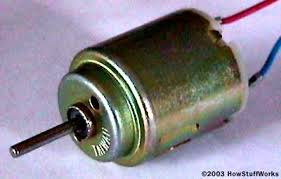
\includegraphics[width=\linewidth]{image6}\\
                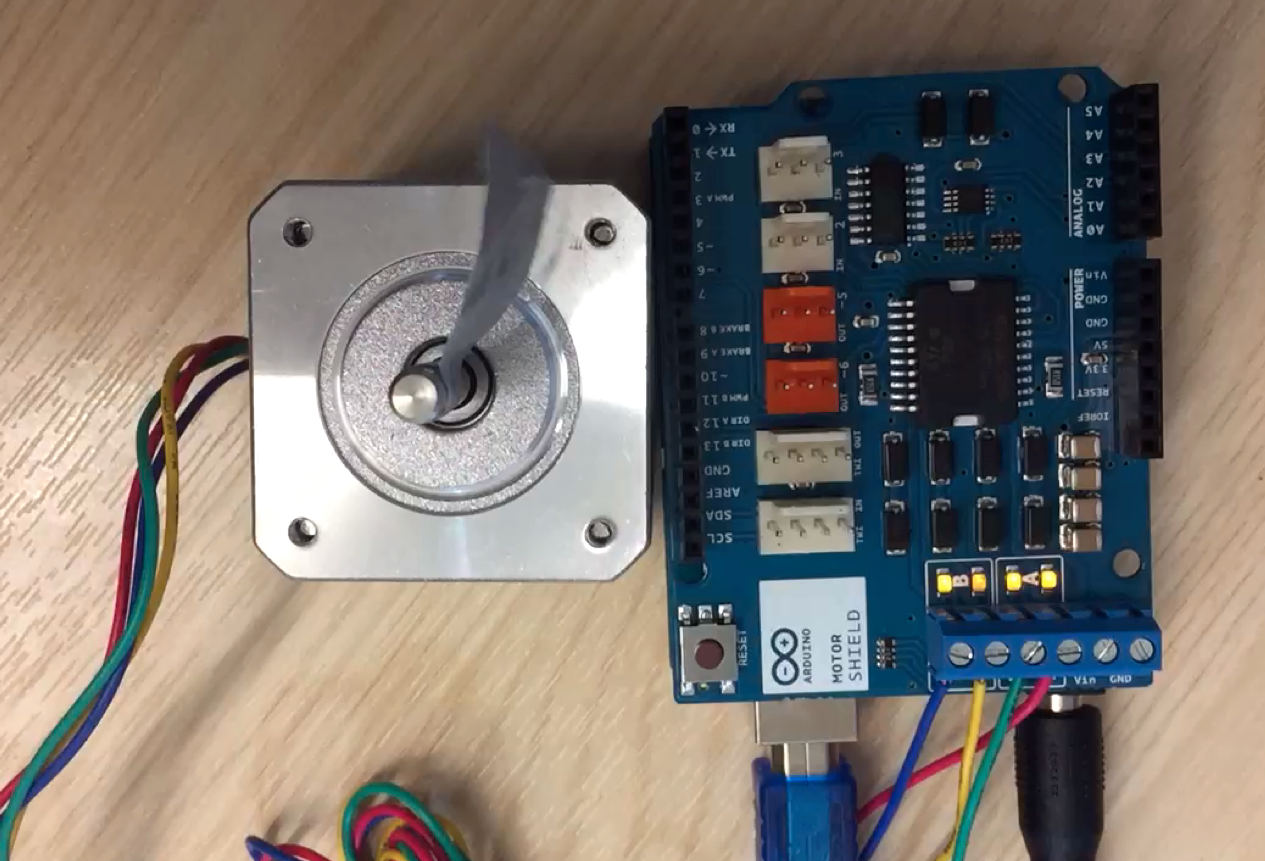
\includegraphics[width=\linewidth]{image7}\\
                \includegraphics[width=\linewidth]{image8}
            \end{center}
        \end{column}
    \end{columns}

\end{frame}

{\fullbackground[scale=0.9]{ian-dc-motors-p3.pdf}
\begin{frame}{Current in magnetic field}
%
%\begin{columns}
%    \begin{column}{0.5\linewidth}
%    A Conductor in a Fixed Magnetic Field
%
%    \textbf{Fixed Magnetic Field}
%
%    \end{column}
%    \begin{column}{0.5\linewidth}
%
%
%    A Current Carrying Conductor in a Fixed Magnetic Field
%
%    Force
%
%    \end{column}
%\end{columns}
%

\end{frame}
}



\begin{frame}[plain]

    \begin{center}
        \bf How simple can it get?
    \end{center}

\end{frame}
\videoframe{part2/figs/homopolarmotor.ogv?start=1}

\begin{frame}{Homopolar Motor}


    \begin{center}
        \begin{tikzpicture}[>=latex]

            \coordinate (anchor) at (0.1,-2.2);
            \node at (0,0) {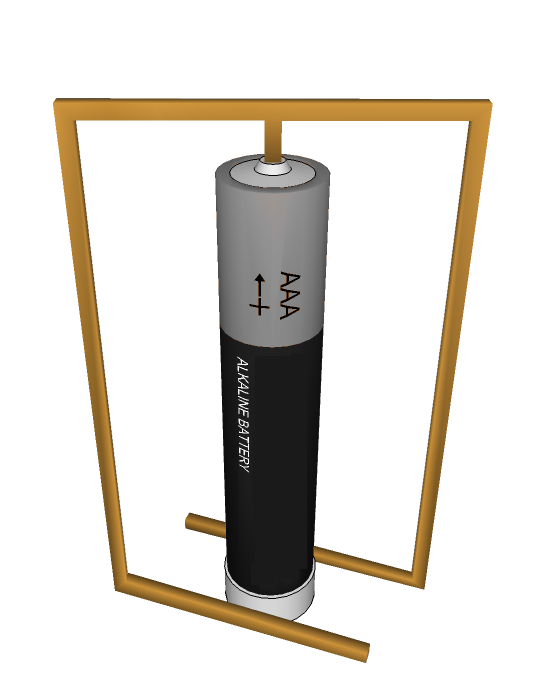
\includegraphics[height=0.6\paperheight]{image10}};
            \node at (1.2,-3.3) (caption) {\footnotesize magnet} edge[bend left,thick,->] (anchor);
        \end{tikzpicture}
        \hspace{2em}
        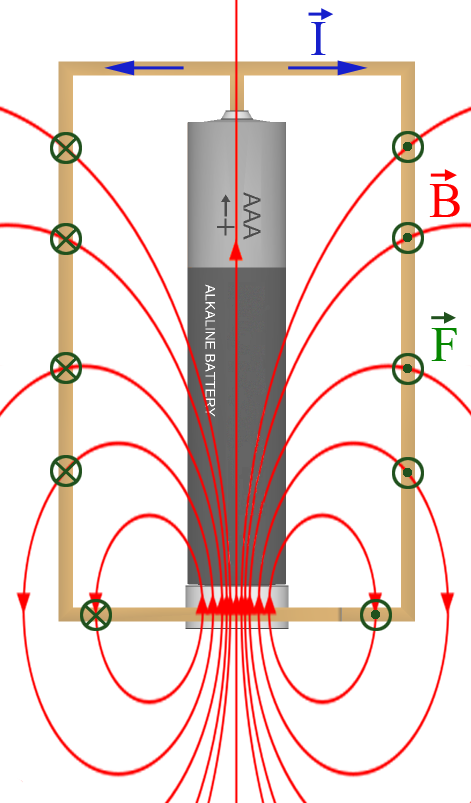
\includegraphics[height=0.6\paperheight]{image11}
    \end{center}

    \source{https://en.wikipedia.org/wiki/Homopolar_motor}{Wikipedia}
\end{frame}

\begin{frame}{Fleming's Left Hand (Motor) Rule}

Used to determine the direction of DC current carrying conductor in a
fixed magnetic field

    \begin{center}
        \resizebox{0.9\linewidth}{!}{
            \begin{tikzpicture}[>=latex]
                \node at (0,0) (hand) {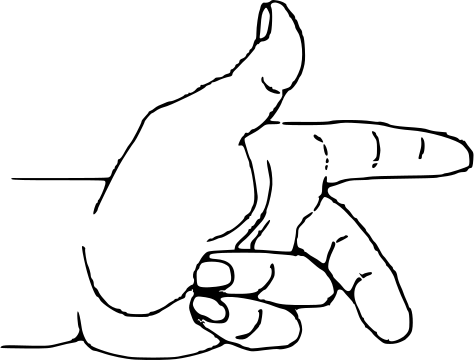
\includegraphics[width=4cm]{left-hand}};
                \coordinate (origin) at (0.45,0.2);

                \draw[ultra thick, ->, blue] (origin) -- ($(origin) + (0,2)$);
                \draw[ultra thick, ->, green] (origin) -- ($(origin) + (2,0)$);
                \draw[ultra thick, ->, red] (origin) -- ($(origin) + (1,-1.4)$);

                \node[below left=2.3 of origin] {\large \bf left hand!};
                \node[align=left,above left=0.7 of origin] {\textbf{Thumb}: \\
                direction of \\ conductor motion};

                \node[align=left,above right=0.5 of origin] {\textbf{Fore
                Finger}:\\ direction of fixed \\magnetic field (N to S)};

                \node[align=left,below right=of origin] {\textbf{Middle
                Finger}:\\ conventional current direction};
            \end{tikzpicture}
        }
    \end{center}




\end{frame}

{\fullbackground[scale=1]{ian-dc-motors-p6.pdf}
\begin{frame}{Using Fleming's Left Hand (Motor) Rule}
%
%The Left Hand Rule to determines the movement direction of conductor
%carrying current
%
%    \begin{center}
%        \resizebox{0.6\linewidth}{!}{
%            \begin{tikzpicture}[>=latex]
%                \node at (0,0) (hand) {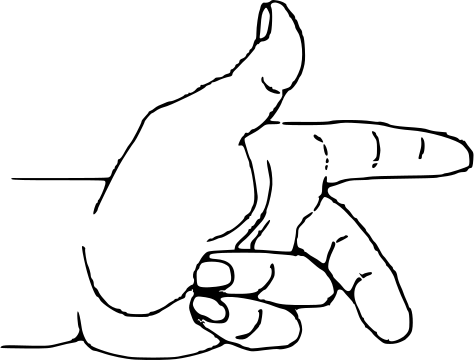
\includegraphics[width=4cm]{left-hand}};
%                \coordinate (origin) at (0.45,0.2);
%
%                \draw[ultra thick, ->, blue] (origin) -- ($(origin) + (0,2)$);
%                \draw[ultra thick, ->, green] (origin) -- ($(origin) + (2,0)$);
%                \draw[ultra thick, ->, red] (origin) -- ($(origin) + (1,-1.4)$);
%
%                \node[below left=2.3 of origin] {\large \bf left hand!};
%                \node[align=left,above left=0.7 of origin] {\textbf{Thumb}: \\
%                direction of \\ conductor motion};
%
%                \node[align=left,above right=0.5 of origin] {\textbf{Fore
%                Finger}:\\ direction of fixed \\magnetic field (N to S)};
%
%                \node[align=left,below right=of origin] {\textbf{Middle
%                Finger}:\\ conventional current direction};
%            \end{tikzpicture}
%        }
%        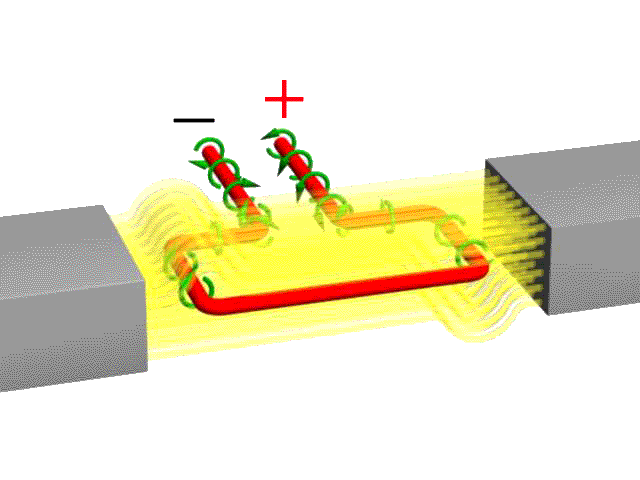
\includegraphics[width=0.6\linewidth]{image13}
%    \end{center}
%
\end{frame}
}

\begin{frame}{Single coil in magnetic field}

    \begin{center}
        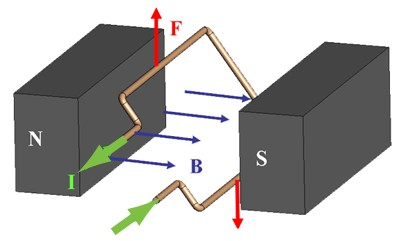
\includegraphics[width=0.5\linewidth]{image15}
    \end{center}

\only<1>{
\begin{itemize}
    \item Current flow results in forces on sections that cut magnetic field
        $\vec{B}$
    \item Left section gets pushed up with force $\vec{F}$
    \item Right section gets pushed down with force $\vec{F}$ where
\[
    \vec{F} = \vec{I} \cdot L \times \vec{B}
\]

\end{itemize}
}

    \only<2>{

In practice the shaft torque of a DC motor is smaller than the
electromagnetic torque because of mechanical losses

\begin{itemize}
    \item Viscous friction will occur in the bearings
    \item Friction arises from the brushes rubbing on the commutator
    \item Air resistance will result in viscous friction due to rotation of the
    armature which may even include a cooling fan
\end{itemize}
}

\end{frame}

\begin{frame}{Cross-section of coil in magnetic field}

    \begin{center}
        \includegraphics<1>[width=0.8\linewidth]{image16-1}
        \includegraphics<2>[width=0.8\linewidth]{image16-2}
        \includegraphics<3->[width=0.8\linewidth]{image16-3}
    \end{center}

\only<3>{
If current $I$ flows through a coil of depth $L$ with magnetic field $B$,
the coil pivots and generates a torque $\tau$ given by:

\begin{equation*}
\begin{split}
\tau = 2 (\frac{d}{2}) \cdot F \cdot cos(\theta) &= d \cdot B \cdot I \cdot L \cdot cos(\theta) \\
                                                 &= d \cdot B \cdot I \cdot L
                                                 \text{\hspace{2em} when } \theta = 0^\circ \\
                                                 &= 0 \text{\hspace{2em} when } \theta = 90^\circ 
\end{split}
\end{equation*}


}

    \only<4>{

        \begin{columns}
            \begin{column}{0.7\linewidth}
                \small
        \begin{itemize}
            \item Moment arm = force $\times$ distance = torque
            \item As the coil rotates, moment arm is reduced and the torque decreases
            \item When the coil is horizontal it is at its maximum value
            \item When the coil is vertical it is zero
            \item NB: torque changes sign as we rotate 360°
        \end{itemize}
                
            \end{column}
            \begin{column}{0.3\linewidth}

    \resizebox{\linewidth}{!}{
        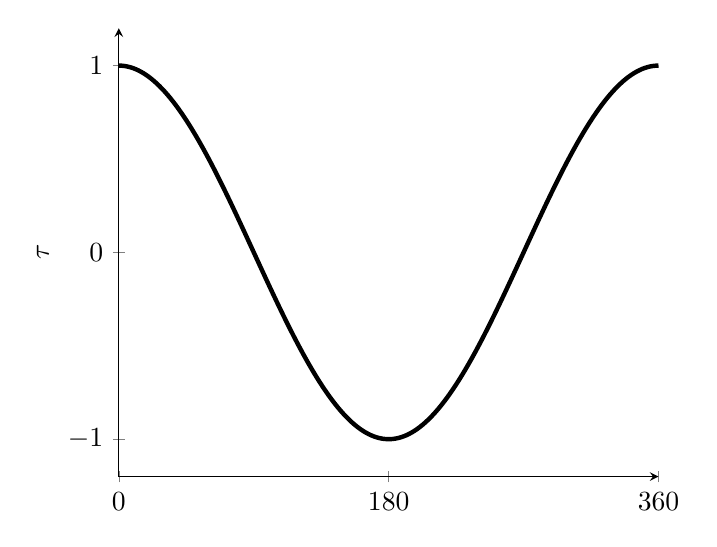
\begin{tikzpicture} 
            \begin{axis}[
                    xtick distance=180,
                    ytick distance=1,
                    no markers, samples=200,
                    axis x line=bottom,
                    axis y line=left,
                    domain=0:360,
                    ymin=-1.2, ymax=1.2,
                    ylabel=$\tau$
                ]
                \addplot[ultra thick] {cos(x)}; 
            \end{axis}
        \end{tikzpicture} 
    }
            \end{column}
        \end{columns}
}
\end{frame}

\begin{frame}{Commutation}

    \begin{columns}
        \begin{column}{0.3\linewidth}
            So coil of wire with fixed current direction has torque that changes
            sign as it rotates

            \vspace{2em}
            \resizebox{\linewidth}{!}{
                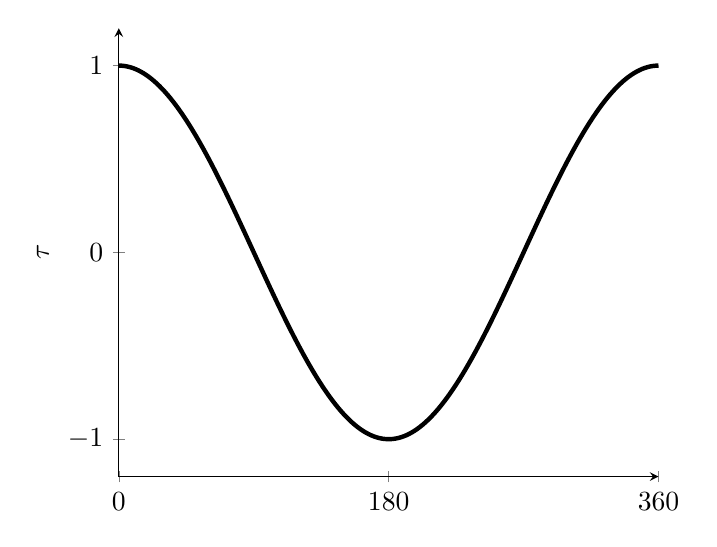
\begin{tikzpicture} 
                    \begin{axis}[
                            xtick distance=180,
                        ytick distance=1,
                        no markers, samples=200,
                        axis x line=bottom,
                        axis y line=left,
                        domain=0:360,
                        ymin=-1.2, ymax=1.2,
                        ylabel=$\tau$
                    ]
                        \addplot[ultra thick] {cos(x)}; 
                    \end{axis}
                \end{tikzpicture} 
            }
        \end{column}
        \begin{column}{0.3\linewidth}
            But we want torque always to be in the same direction!

            So use commutator to switch it!

            \begin{center}
                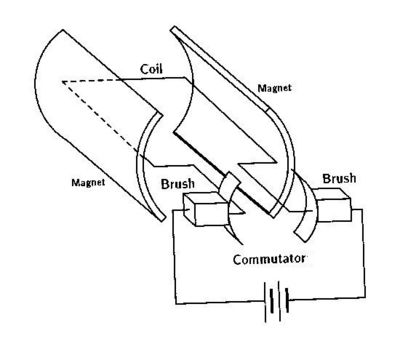
\includegraphics[width=1.2\columnwidth]{image22}
            \end{center}
        \end{column}
        \begin{column}{0.3\linewidth}

            Switching current direction before torque direction flips ensures
            that it is always in same direction
            
            \vspace{2em}
            \resizebox{\linewidth}{!}{
                \begin{tikzpicture} 
                    \begin{axis}[
                            xtick distance=180,
                        ytick distance=1,
                        no markers, samples=200,
                        axis x line=bottom,
                        axis y line=left,
                        domain=0:360,
                        ymin=-1.2, ymax=1.2,
                        ylabel=$\tau$
                    ]
                        \addplot[ultra thick] {abs(cos(x))}; 
                    \end{axis}
                \end{tikzpicture} 
            }
        \end{column}
    \end{columns}



\end{frame}

\begin{frame}{Precious metal commutators}

    \begin{columns}
        \begin{column}{0.6\linewidth}
            \begin{itemize}
                \item Well suited for smallest currents and~voltages
                \item Well suited for continuous operation
                \item Smaller motors
                \item Very low friction
                \item Low audible noise
                \item Low electromagnetic interference
                \item Cost effective
                \item Not suited for high current and peak currents
                \item Not suited for start-stop operation
            \end{itemize}

        \end{column}
        \begin{column}{0.4\linewidth}
            \begin{center}
                \resizebox{\linewidth}{!}{
                    \begin{tikzpicture}[>=latex]

                        \coordinate (anchor) at (-1.9,-0.1);
                            \node at (0,0) {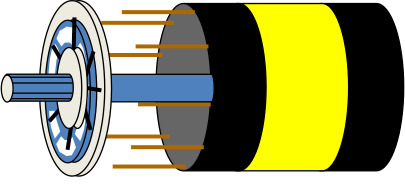
\includegraphics[width=\linewidth]{precious-metal-commutators}};
                            \node at (-0.2,-2) (caption) {\footnotesize silver commutator} edge[bend left,thick,->] (anchor);
                    \end{tikzpicture}
                }
            \end{center}
        \end{column}
    \end{columns}

\end{frame}

\begin{frame}{Carbon brush commutators}
    \begin{columns}
        \begin{column}{0.6\linewidth}

            Graphite brushes

            \begin{itemize}
                \item Well suited for high currents and peak currents
                \item Well suited for start-stop and reversing operation
                \item Larger motors ($>$ approx. 10 W)
                \item Higher friction
                \item Higher no-load current
                \item Not suited for small currents
                \item Higher audible noise
                \item Higher electromagnetic emissions
                \item Higher costs
            \end{itemize}

        \end{column}
        \begin{column}{0.4\linewidth}

            \begin{center}
                \resizebox{\linewidth}{!}{
                    \begin{tikzpicture}[>=latex]

                        \coordinate (anchor) at (-1.5,0);
                            \node at (0,0) {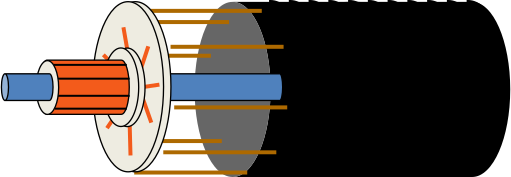
\includegraphics[width=\linewidth]{carbon-brush-commutators}};
                            \node at (0,-1.5) (caption) {\footnotesize copper
                            commutator} edge[bend left,thick,->] (anchor);
                    \end{tikzpicture}
                }

                \vspace{2em}
                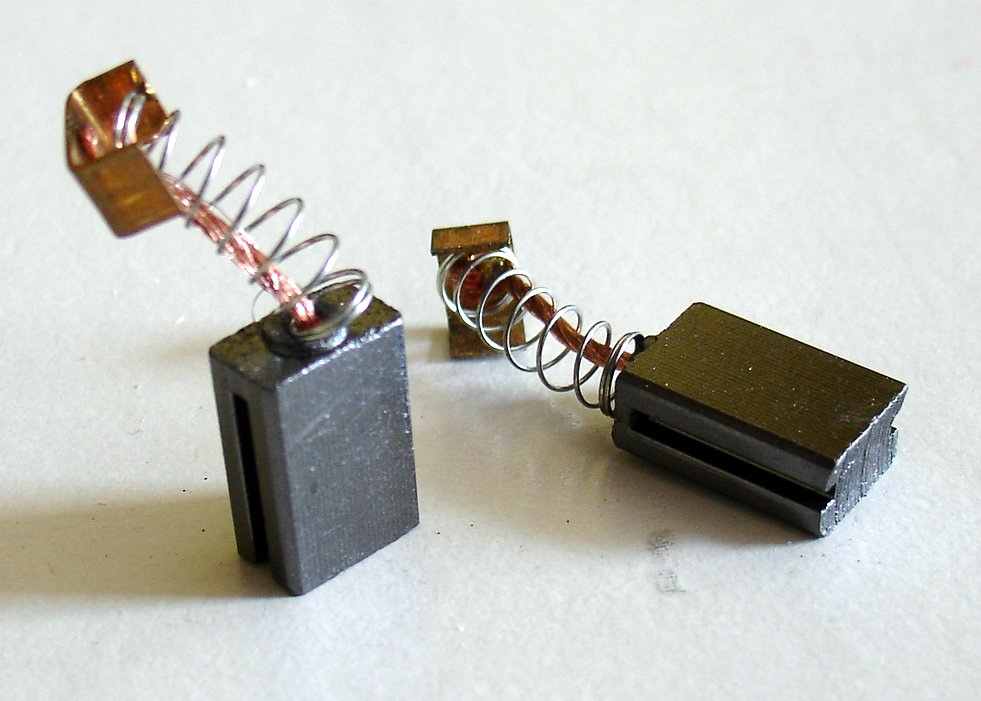
\includegraphics[width=0.8\linewidth]{image23}
            \end{center}
        \end{column}
    \end{columns}


\end{frame}

\begin{frame}{DC Motor Torque Ripple}

    \begin{center}
        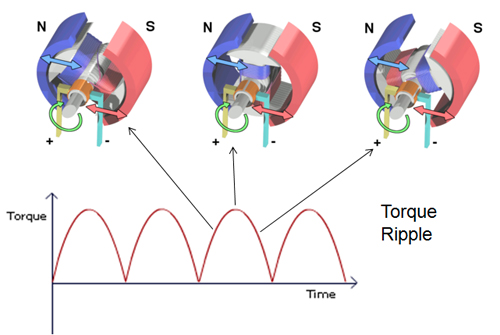
\includegraphics[height=0.4\paperheight]{image24}\hspace{1em}
        \video[1]{0.35\linewidth}{part2/figs/torque-ripple.mp4?autostart&loop}
    \end{center}

\begin{itemize}
\item With single coil the torque still drops to zero when the coil is
  vertical
\item This fluctuation is known as torque ripple
\item However with torque always in same direction coil will now rotate
  continuously
\end{itemize}

\end{frame}

\begin{frame}{Multiple coils reduces torque ripple}

    \begin{columns}
        \begin{column}{0.5\linewidth}
            \begin{center}
                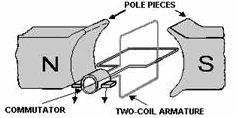
\includegraphics[width=\linewidth]{image26}

                \vspace{2em}

                \footnotesize Overall torque summed from both coils

                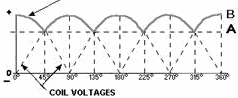
\includegraphics[width=\linewidth]{image26-2}

            \end{center}
        \end{column}
        \begin{column}{0.5\linewidth}

            \begin{center}
                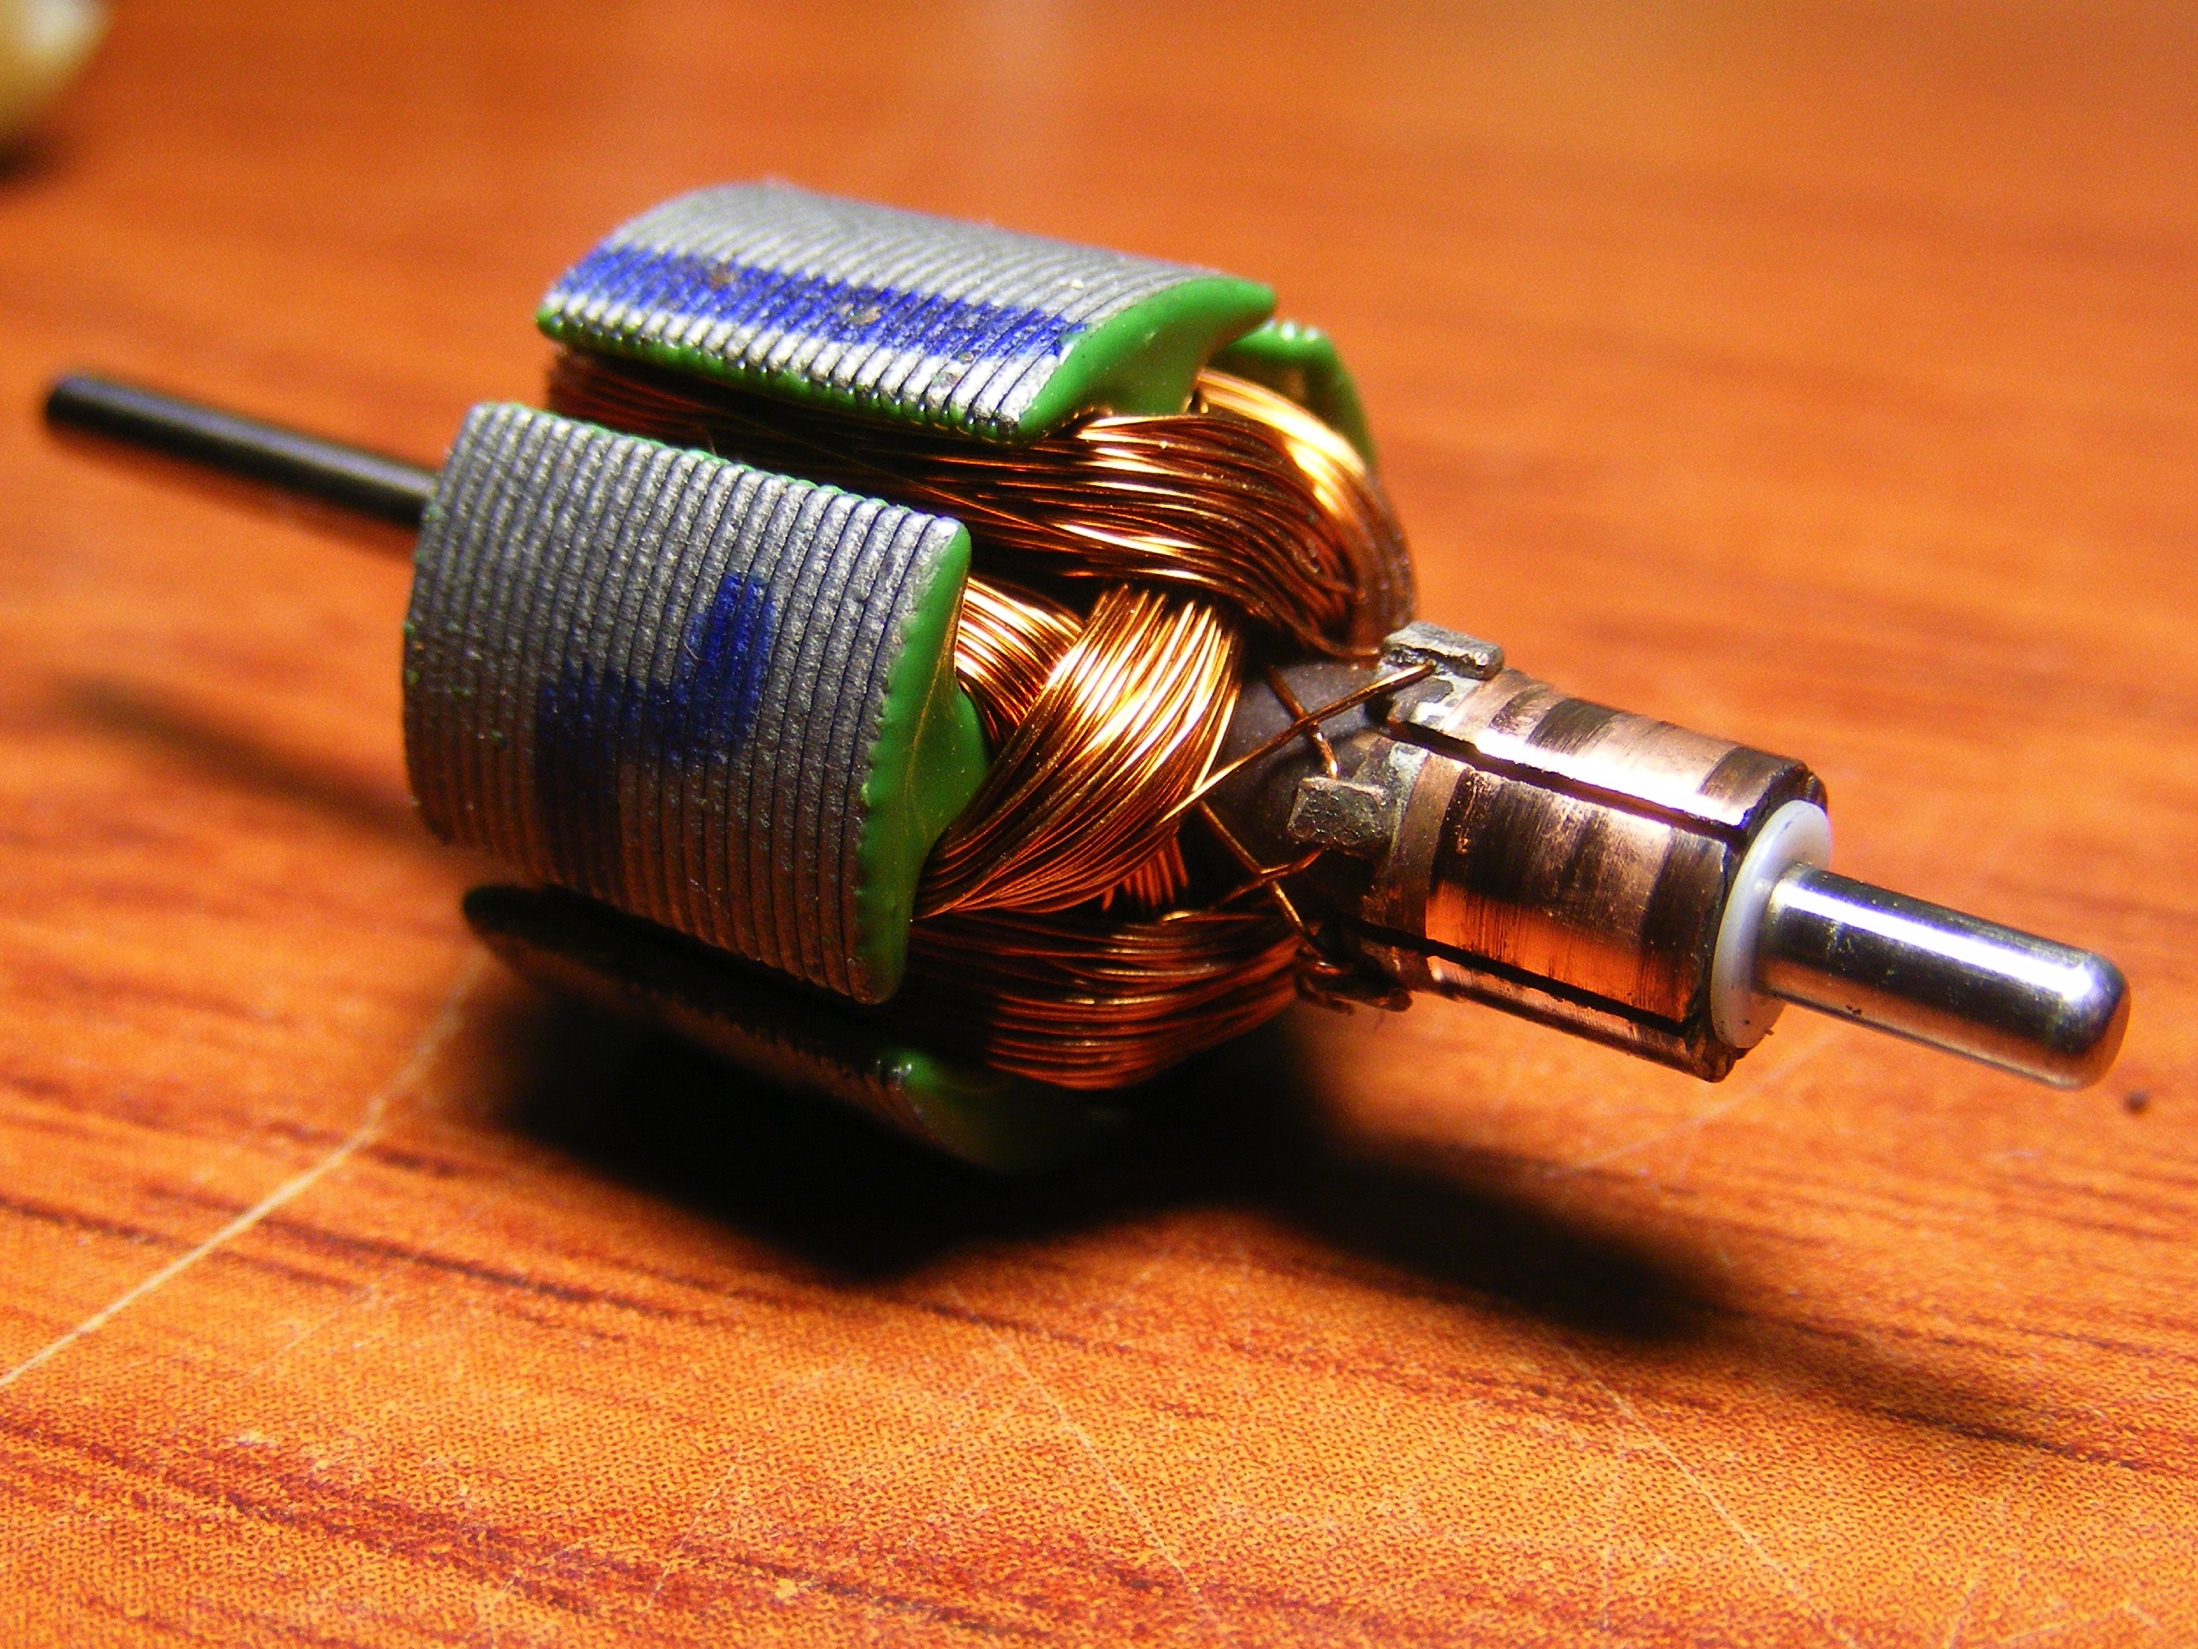
\includegraphics[width=0.8\linewidth]{image27}

                Typical small armature with multiple multi-turn coils
            \end{center}
        \end{column}
    \end{columns}


\end{frame}

\begin{frame}{Remember electromagnetic induction}

  Moving a magnet in a coil induces current


    \begin{center}
        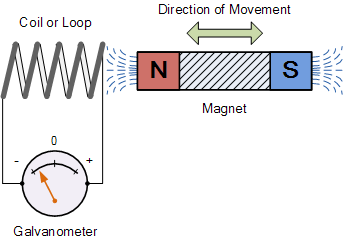
\includegraphics[width=0.6\linewidth]{image29}

    \scalebox{1.5}{Faraday's law of induction: $\displaystyle\mathcal{E} = -N \cdot \frac{d\Phi_B}{dt}$}

    \end{center}
\end{frame}

\begin{frame}{Electrical generator}

    \begin{center}
        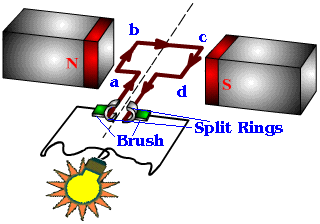
\includegraphics[width=0.6\linewidth]{image30}
    \end{center}

\begin{itemize}

\item Speed of rotation affects voltage generated
\item So how fast will a motor rotate with applied voltage $V$?
\item Lets consider the equivalent circuit for a DC motor
\end{itemize}
\end{frame}

\begin{frame}{DC motor equivalent circuit}

    \begin{center}
        \resizebox{0.6\linewidth}{!}{
            % Based on http://texample.net/tikz/examples/induction-machine/
            \begin{circuitikz}
                \draw
                % rotor circuit
                (0,0) to [short, *-] (6,0)
                to [V, l_={EMF: $\mathrm{j}{\omega}_m \psi$}] (6,2) % rotor emf

                % stator circuit
                (0,0) to [open, v^>=$V$] (0,2) % stator voltage
                to [short, *- ,i=$I$] (1,2) % stator current
                to [R, l=$R$] (3,2) % stator resistance
                to [L, l=$L$] (6,2); % leakage inductance
            \end{circuitikz}
        }
    \end{center}

\footnotesize
\begin{itemize}

\item $V$ is the applied voltage, $I$ is the drawn current
\item Resistance $R$ arises from the coil and the brushes
\item Inductance $L$ arises from the coil
\item Back EMF arises from rotation of the coil in the magnetic field
  created by the stator magnets
\item Therefore in no-load condition motor will speed up and reach steady
  state when: $V$ = back EMF
\end{itemize}

\end{frame}

\begin{frame}{DC motor as an energy converter}


\begin{itemize}

\item Can also use the equivalent circuit to estimate energy conversion
\item Converts electrical energy into mechanical energy + heat
\item Electrical power in = voltage i$\times$ current
\item Mechanical power out = Speed ($rad \cdot s^{-1}$) $\times$ torque (NM)
\end{itemize}

    \begin{columns}
        \begin{column}{0.7\linewidth}
    \begin{center}
        \resizebox{0.9\linewidth}{!}{
            \begin{tikzpicture}[>=latex]

                \node at (0,0) (motor) {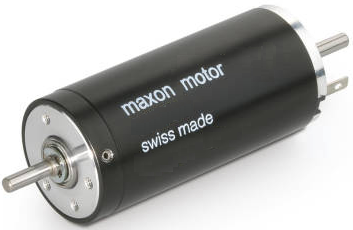
\includegraphics[width=3cm]{maxon}};
                \node[below left=0.5 of motor] (pmech) {$P_{mech}=2\pi\frac{n}{60}\cdot \tau$};
                \node[above right=0.5 of motor] (pel) {$P_{el}=V \cdot I$};
                \node[below right=0.5 of motor] (pr) {$P_{r}=R \cdot I^2$};
                \draw[ultra thick, red,->] (motor) -- (pmech);
                \draw[ultra thick, red,->] (pel) -- (motor);
                \draw[ultra thick, orange,->] (motor) -- (pr);
            \end{tikzpicture}
        }

    \[
        P_{el} = P_{mech} + P_{r} = V\cdot I = 2\pi\frac{n}{60}\cdot \tau + I^2 R
    \]
    \end{center}

        \end{column}
        \begin{column}{0.3\linewidth}
    \footnotesize
    where:

        $\tau$ = torque;
        
        $N$ = rotation speed in rpm;
        
        $I$ = input current;
        
        $V$ = applied voltage
            
        \end{column}
    \end{columns}

\note{

In a very general frame motors can be considered as energy converters.
DC motors convert the electrical input power (DC voltage V and current
I) into mechanical output power consisting of angular speed ω and torque
M. Engineers prefer to use rotational speed n measured in rpm instead of
rad/s; that's why there is a factor of π/30 to get the unit of power
right in Watts.

The theory described in this presentation applies to any DC motor, in
particular to the maxon DC motor and the brushless maxon EC motor.
}

\end{frame}

\section{Simple DC motor construction}

\begin{frame}{Basic parts of a brushed DC motor}

\begin{columns}
    \footnotesize
    \begin{column}{0.5\linewidth}
    \begin{itemize}
        \item Bearings are mounted each end of the output shaft
        \item Housing provides support for the bearings and holds the stator magnets
        \item It also provides protection and mechanical attachment
        \item Armature may have skewed coil slots to reduce cogging
    \end{itemize}

    \resizebox{\columnwidth}{!}{
    \begin{tikzpicture}[>=latex]
        \node at (0,0) {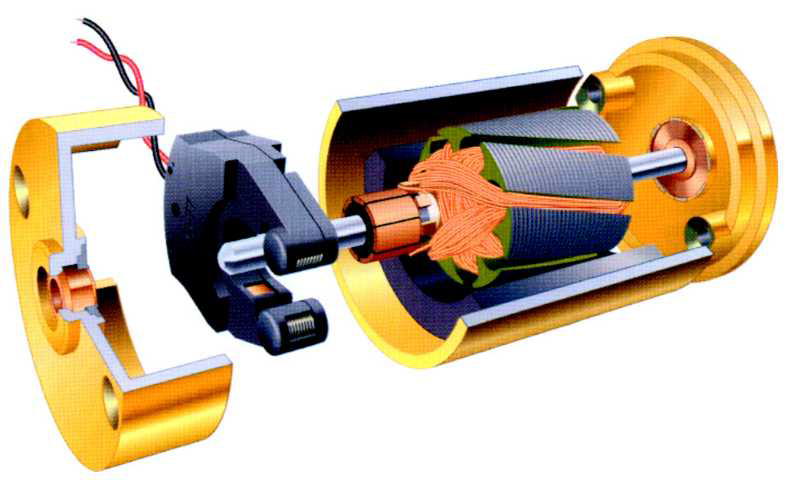
\includegraphics[width=0.9\columnwidth]{image39}};
        \node at (-2,1.5) {\footnotesize brushes} edge[bend left,thick,->] (-1.2,0.5);
        \node at (-0.5,1.5) {\footnotesize housing} edge[bend left,thick,->] (0.5, 1);
        \node at (2,1.5) {\footnotesize bearings} edge[bend left,thick,->] (1.7, 0.7);
        \node at (0,-1.3) {\footnotesize commutator} edge[bend left,thick,->] (0,0);
        \node at (2,-1) {\footnotesize laminated iron core} edge[bend left,thick,->] (1,0);
    \end{tikzpicture}
    }


    \end{column}
    \begin{column}{0.5\linewidth}
    \begin{itemize}
        \item Stator magnets generate magnetic field so current in coils generate
        toque
        \item Armature rotor consists of laminated iron core wrapped with coils to
        give mow reluctance but avoid eddy current
        \item Commutator used so switch current direction and permit continuous
        rotation
        \item Brushes provide contact to commutator
    \end{itemize}


    \resizebox{\columnwidth}{!}{
        \begin{tikzpicture}[>=latex]
            \node at (0,0) {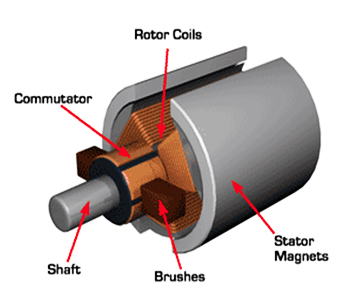
\includegraphics[width=0.9\columnwidth]{image38}};
        \end{tikzpicture}
    }


    \end{column}
\end{columns}
\end{frame}

\imageframe[color=black,caption=Typical example of commutated armature]{image40}


\begin{frame}{Coreless Maxon DC motor (RE 35)}

    \resizebox{\columnwidth}{!}{
        \begin{tikzpicture}[>=latex]
            \node at (0,0) {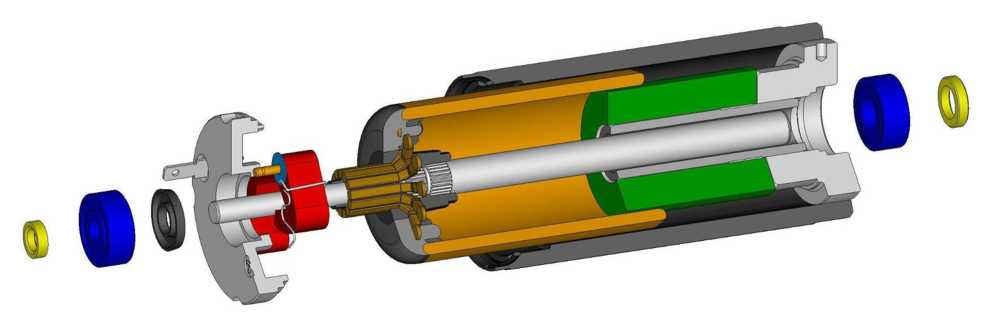
\includegraphics[width=0.9\columnwidth]{image41}};
            \node at (-4.7,-1.5) {\footnotesize press ring} edge[thick,->] (-4.5,-0.9);
            \node at (-3.8,-2) {\footnotesize ball bearing} edge[thick,->] (-3.8,-1.1);
            \node at (-4,0.3) {\footnotesize el. connections};
            \node at (-3,1) {\footnotesize brushes} edge[bend left,thick,->] (-1.8,0);
            \node at (-1.5,-2) {\footnotesize commutator} edge[bend left,thick,->] (-1.2,-0.2);
            \node at (-2,1.5) {\footnotesize commutator plate} edge[bend left,thick,->] (-1.2,0.5);
            \node at (-1,2) {\footnotesize self supporting winding} edge[bend left,thick,->] (-0.5,0.6);
            \node at (0.5,1.5) {\footnotesize shaft} edge[thick,->] (0.5,0);
            \node[minimum width=2cm,align=center] at (1,-1.5) {\footnotesize permanent magnet\\ \footnotesize(in the centre)} edge[bend right,thick,->] (2,-0.2);
            \node[minimum width=2cm,align=center]  at (3,-2) {\footnotesize housing\\ \footnotesize (magnetic return)} edge[bend right,thick,->] (2.5,-0.5);
            \node at (4,-0.8) {\footnotesize flange} edge[bend right,thick,->] (3.5,-0.2);
            \node at (3,2) {\footnotesize ball bearing} edge[bend left,thick,->] (3.8,0.9);
            \node at (3.6,2.5) {\footnotesize press ring} edge[bend left,thick,->] (4.5,0.9);

            %\grid{}
        \end{tikzpicture}
    }



\note{
This picture shows a coreless maxon DC motor. We recognize the same
three subassemblies as with the conventional motor.

The \textbf{stator} consists of the permanent magnet at the centre (here
shown in green), of the housing (again serving as the magnetic return)
and of the mounting flange.

The \textbf{rotor} with winding and commutator. The winding is connected
to the shaft by the so called commutator plate. In this example the
shaft is supported in the stator by ball bearings. The shape of the
rotor reminds of a Xmas bell; that's why it is sometimes called ``bell
shaped'' armature. The winding moves in the air gap between magnet and
housing.

The \textbf{brush system} here with graphite brushes in red and with the
electrical motor connections.

The next slides show the advantages of a ironless motor design.
}

\end{frame}

\begin{frame}{Magnetic circuit of the Maxon Stator}

    \resizebox{\linewidth}{!}{
        \begin{tikzpicture}[>=latex]
            \node at (0,0) {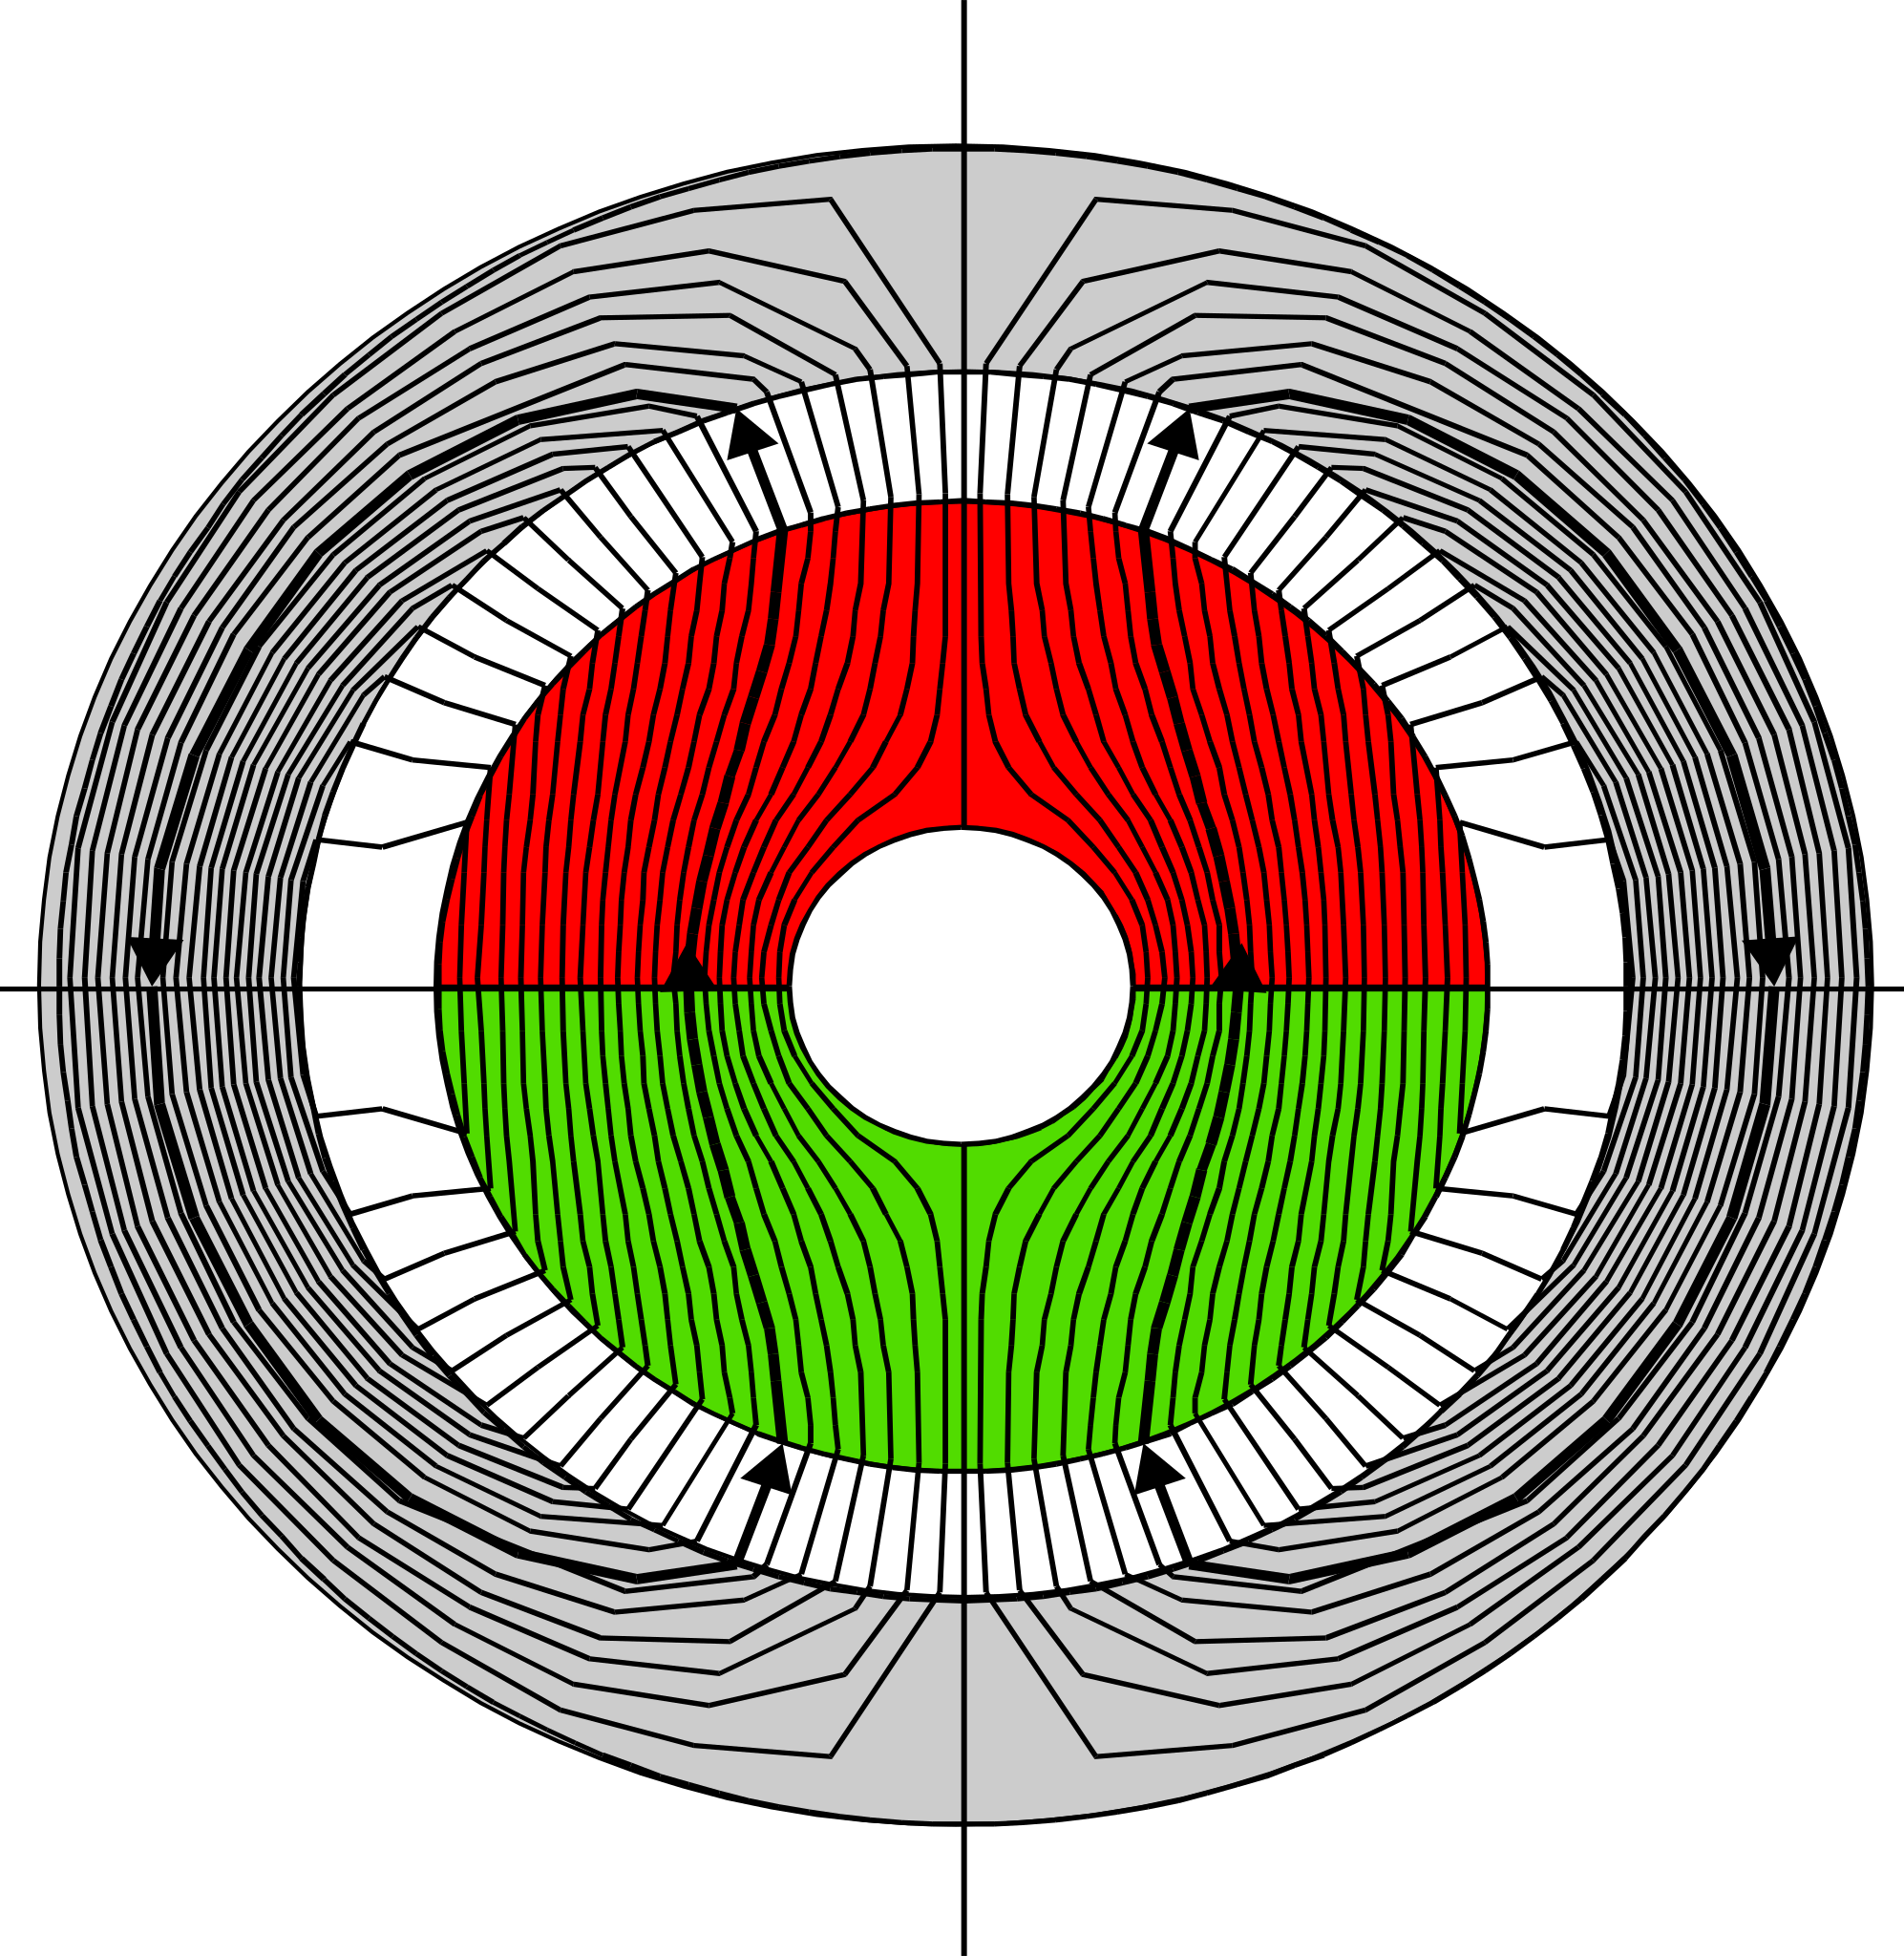
\includegraphics[width=0.5\linewidth]{maxon_stator}};

            \node[minimum width=2cm,align=left,anchor=west] at (3,2) {\footnotesize \textbf{Housing}\\ magnetic return path made\\ of magnetic steel (iron)\\ guides magnetic field} edge[bend right,thick,->] (1.5,1.5);
            \node[minimum width=2cm,align=left,anchor=west]  at (3.5,0) {\footnotesize \textbf{Air gap}\\ the larger the air gap, \\the weaker the magnetic field} edge[thick,->] (1.8,0.5);
            \node[minimum width=2cm,align=left,anchor=west]  at (3,-2) {\footnotesize \textbf{Permanent magnet}\\ produces the magnetic field \\with north and south pole \\on opposite sides} edge[bend left,thick,->] (0.5,-0.5);
            %\grid{}
        \end{tikzpicture}
    }

\note{

After this introduction let's now consider the magnetic circuit in the
stator in more detail.

This slides shows a cross section of the stator.

In the centre we have the \textbf{permanent magnet}. It is diametrically
magnetized, the north pole being colored in red, the south pole in
green. The bore in the middle serves for the motor shaft.

The \textbf{magnetic field lines} leave the magnet at the north pole and
enter the magnet at the south pole. Magnetic field lines - more exactly
the magnetic induction B - are closed lines and must be guided back from
the north to the south pole. That's the duty of the housing which is
made of a magnetically conducting material. That's why the housing is
also called \textbf{magnetic return}.

Between the permanent magnet and the magnetic return the field lines
point in radial direction in the \textbf{air gap}. The goal of this
arrangement is to create an magnetic field as strong as possible in the
air gap in order for the winding to produce as much force as possible.
Air is a bad magnetic conductor and the larger the air gap the smaller
the magnetic flux that can be built. That's why the air gap should be as
narrow as possible. However in a narrow air gap there is room for only a
thin walled winding. The current density is small and so is the produced
force. We see that finding the right dimensions for the air gap is a
classic optimization problem depending strongly on the properties of the
permanent magnet.

In short: We have a configuration producing a magnetic field in the air
gap which points from bottom to top in this representation.

}

\end{frame}

\begin{frame}{Maxon DC motors versus conventional motors}

    \begin{columns}
        \begin{column}{0.5\linewidth}

            \begin{center}
                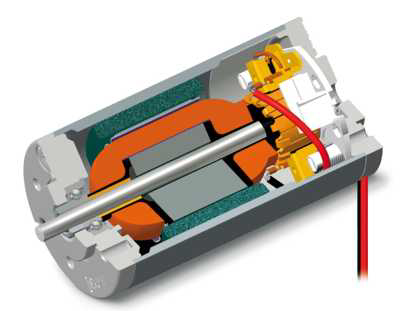
\includegraphics[width=0.8\columnwidth]{image46}
            \end{center}

Conventional motor with rotating magnet and iron core

\begin{itemize}

\item Detent torque (cogging)
\item Inefficient, iron core losses
\item Large physical size
\item High inertia
\end{itemize}

        \end{column}
        \begin{column}{0.5\linewidth}

            \begin{center}
                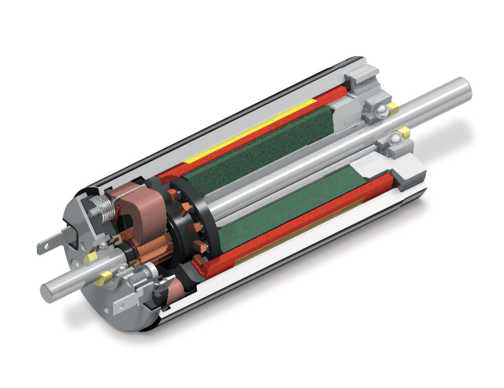
\includegraphics[width=0.8\columnwidth]{image45}
            \end{center}


Maxon motor with stationary magnet and special winding

\begin{itemize}
\item Smooth
\item Linear Characteristic
\item Efficient
\item Responsive
\item Powerful
\end{itemize}

        \end{column}
    \end{columns}

\end{frame}

\begin{frame}{Advantage of coreless armature}

\begin{columns}
    \begin{column}{0.6\linewidth}

\begin{itemize}

\item No iron core - no iron losses
\item Constantly impressed magnetization
\item High efficiency, up to over 90\%
\item No saturation effects in the iron core
\item Even at the highest currents the produced torque is proportional to
  the motor current
\item Stronger magnets = stronger motors
\end{itemize}

    \end{column}
    \begin{column}{0.4\linewidth}

        \begin{center}
            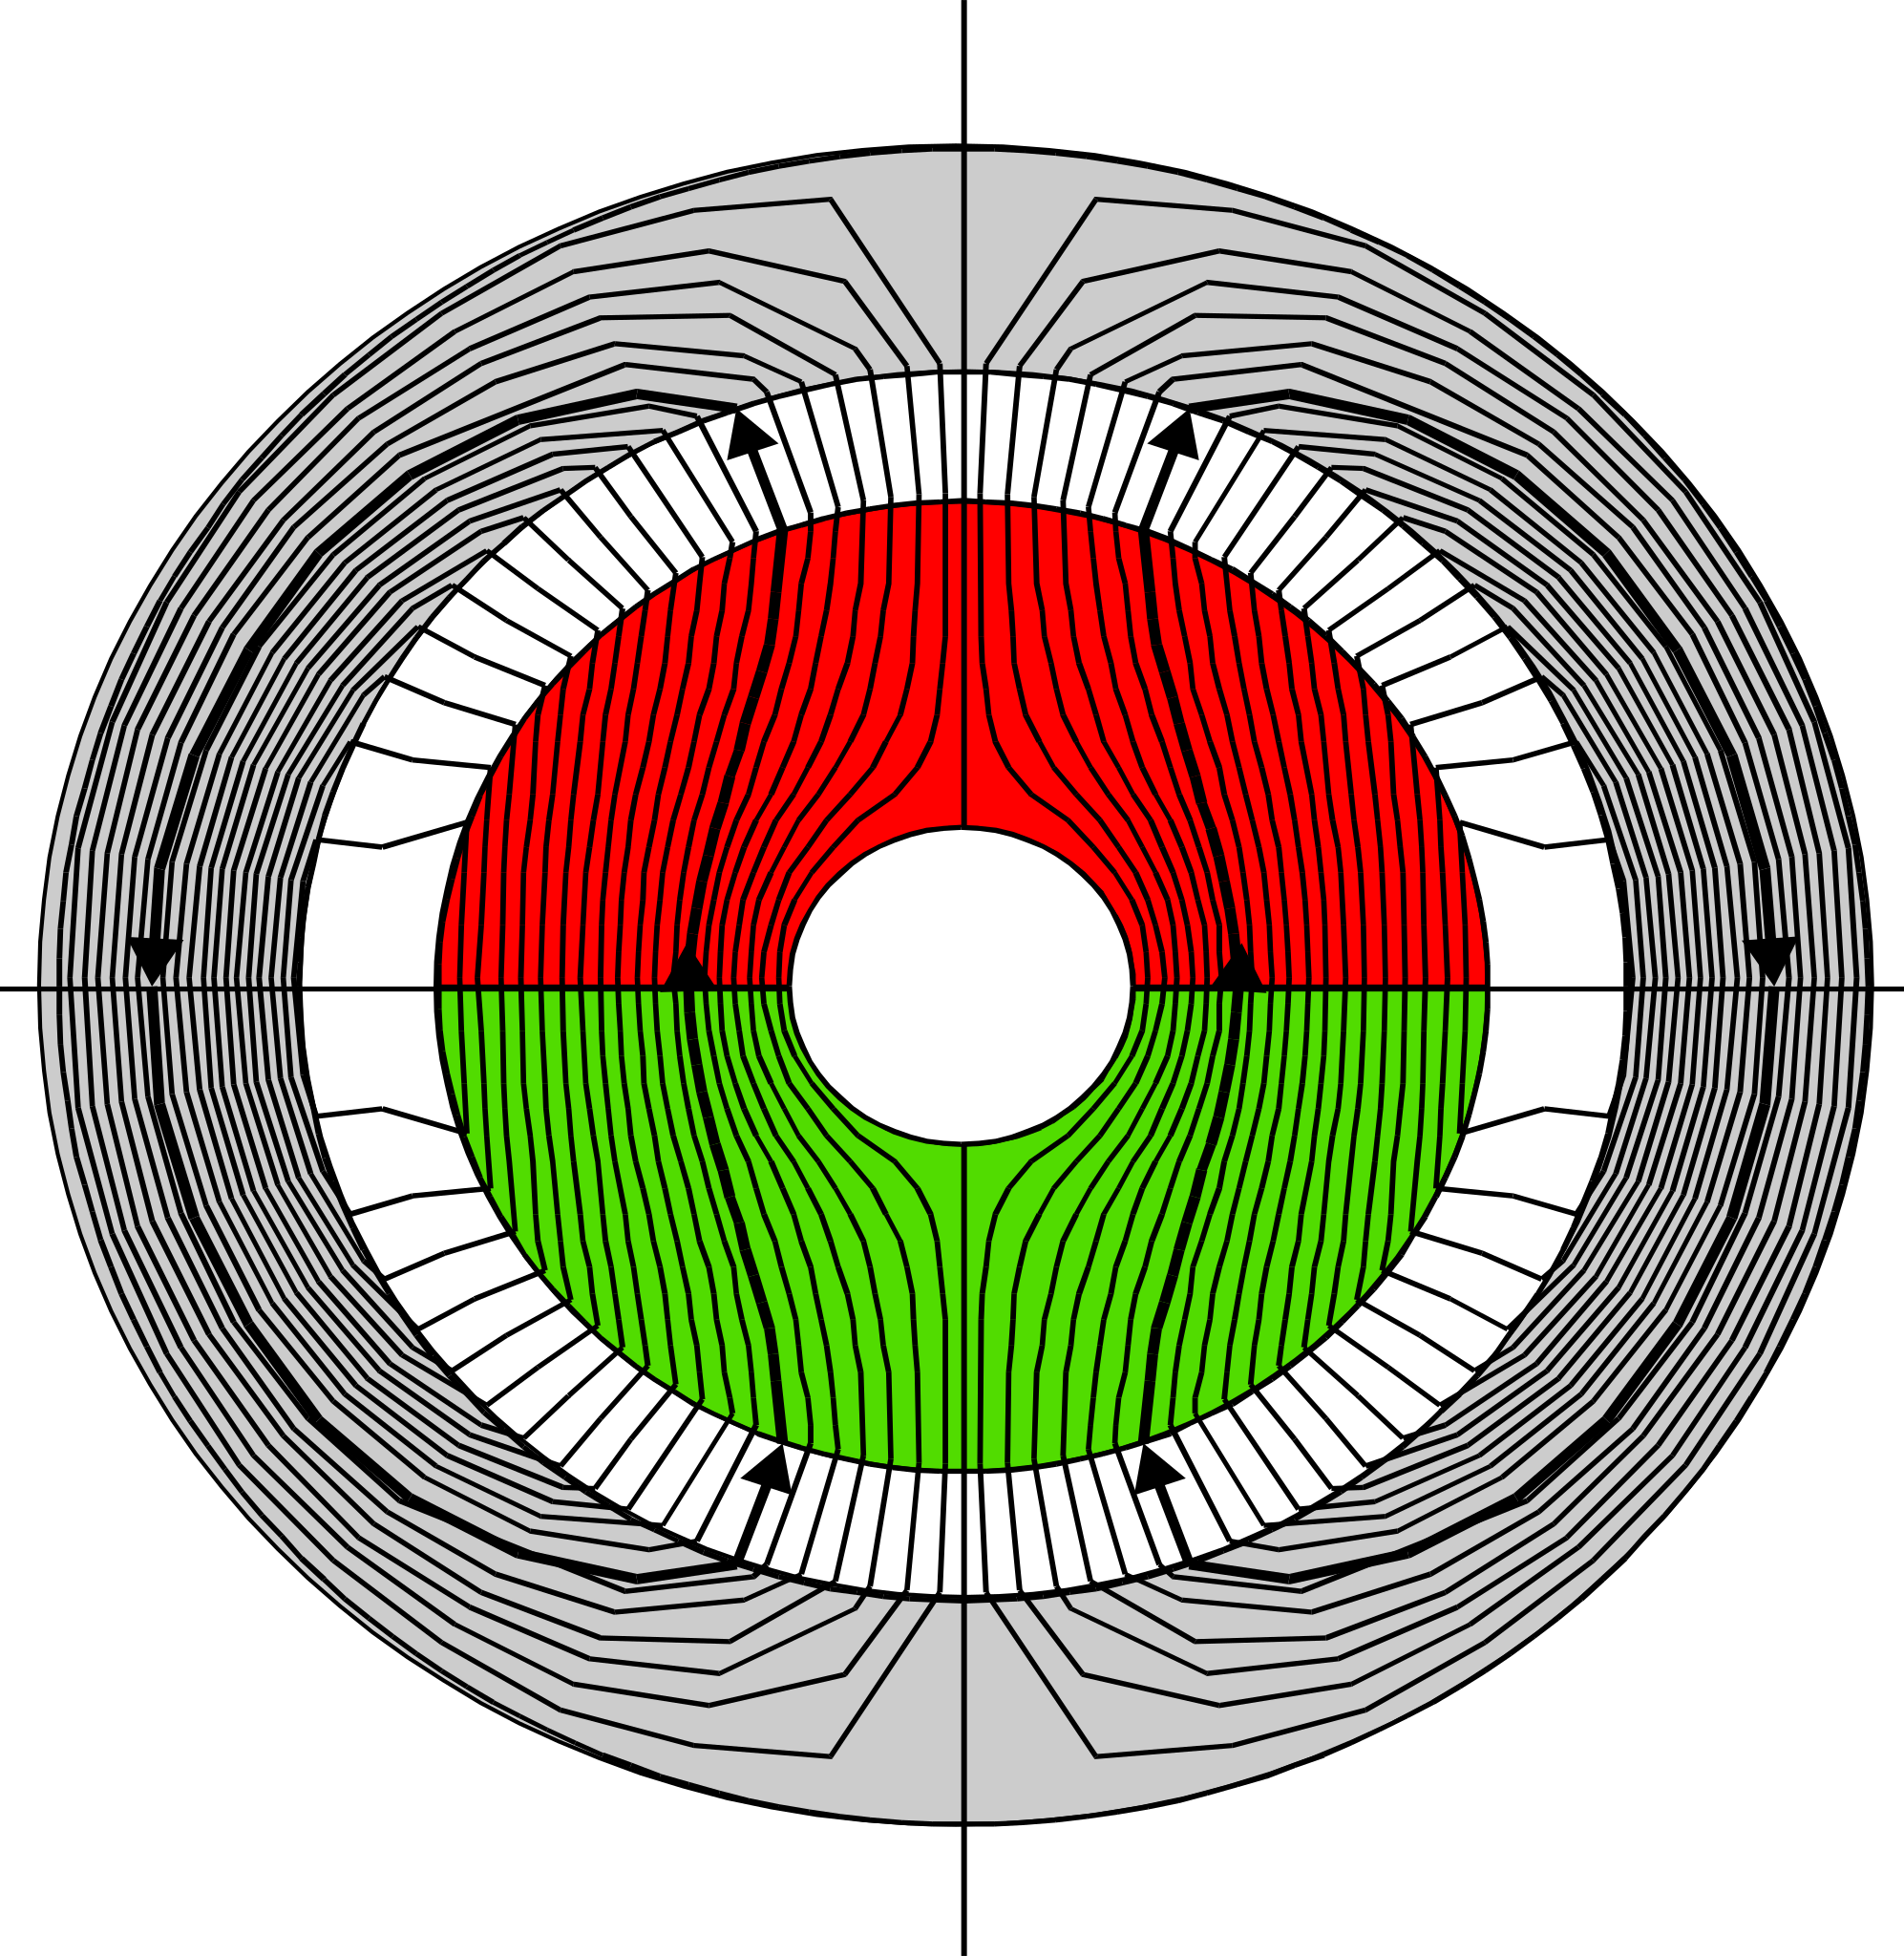
\includegraphics[width=0.8\columnwidth]{maxon_stator}
        \end{center}
    \end{column}
\end{columns}

    \note{

Coreless DC motors have \textbf{no iron losses}.

In a conventional design the iron core permanently changes its
magnetization. This consumes energy because the magnetic hysteresis loop
must be run through at each shaft rotation. Additionally these flux
variations induce Eddy currents in the iron core resulting in power
losses that grow with the square of the motor speed.

By contrast, in a coreless motor the Magnetization is permanently
impressed and constant. (The influence of the magnetic field of the
winding can be neglected in a first approximation.) Hence there are no
iron losses. As a result, the power losses are smaller, the
\textbf{efficiency is higher} and the \textbf{no-load current is lower}.

In an ironless design \textbf{no saturation} at the narrow parts of the
iron core (at the base of the teeth) can occur. Hence the produced
torque remains \textbf{exactly proportional} to the motor current and
one can use the strongest permanent magnets without being limited by the
maximum magnetic flux in the iron core. Improvements in magnet
technology lead to \textbf{stronger motors}.

}

\end{frame}

\begin{frame}{2 and 4 pole motors}

    We don't need to limit number of poles to two

    \begin{columns}
        \begin{column}{0.5\linewidth}
            \begin{center}
                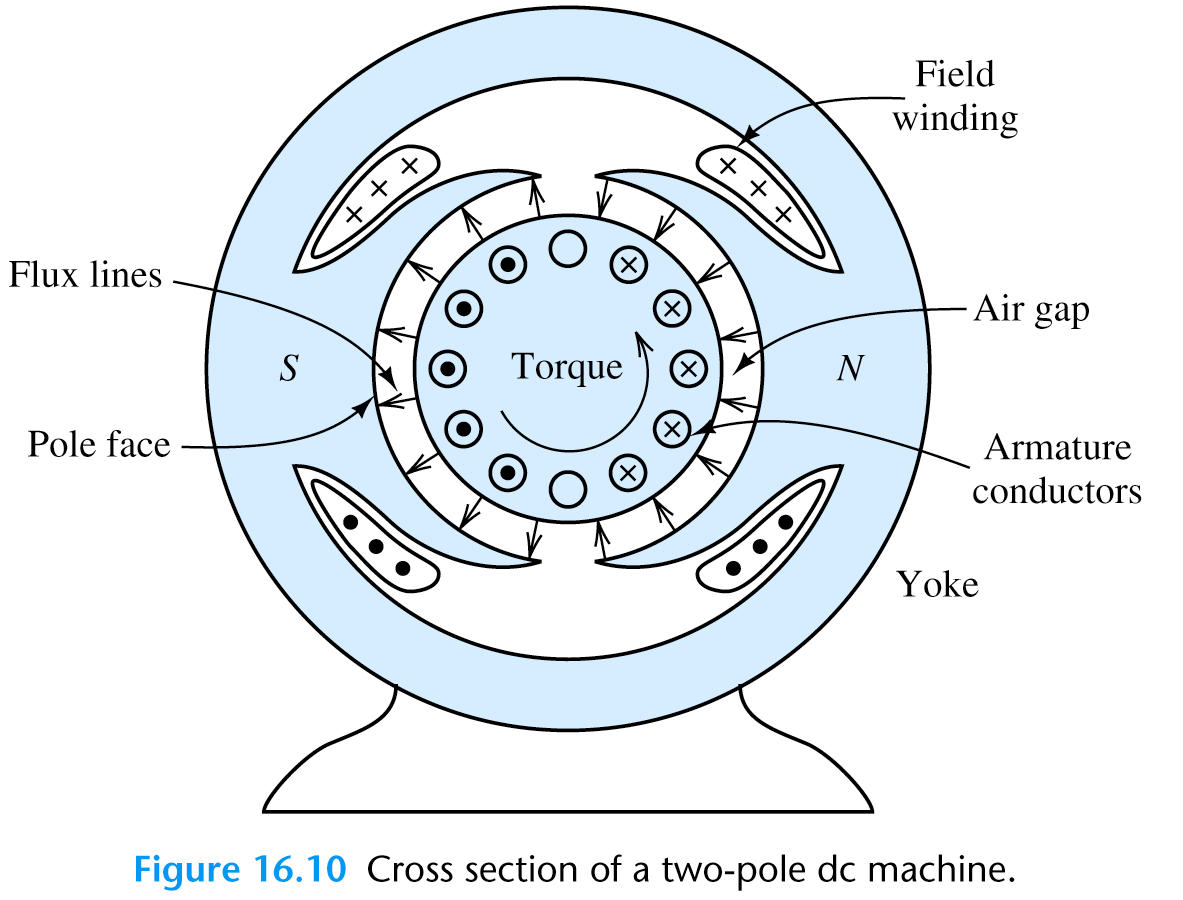
\includegraphics[height=0.5\paperheight]{image48}

                \textbf{2 pole motors}
            \end{center}
        \end{column}
        \begin{column}{0.5\linewidth}

            \begin{center}
                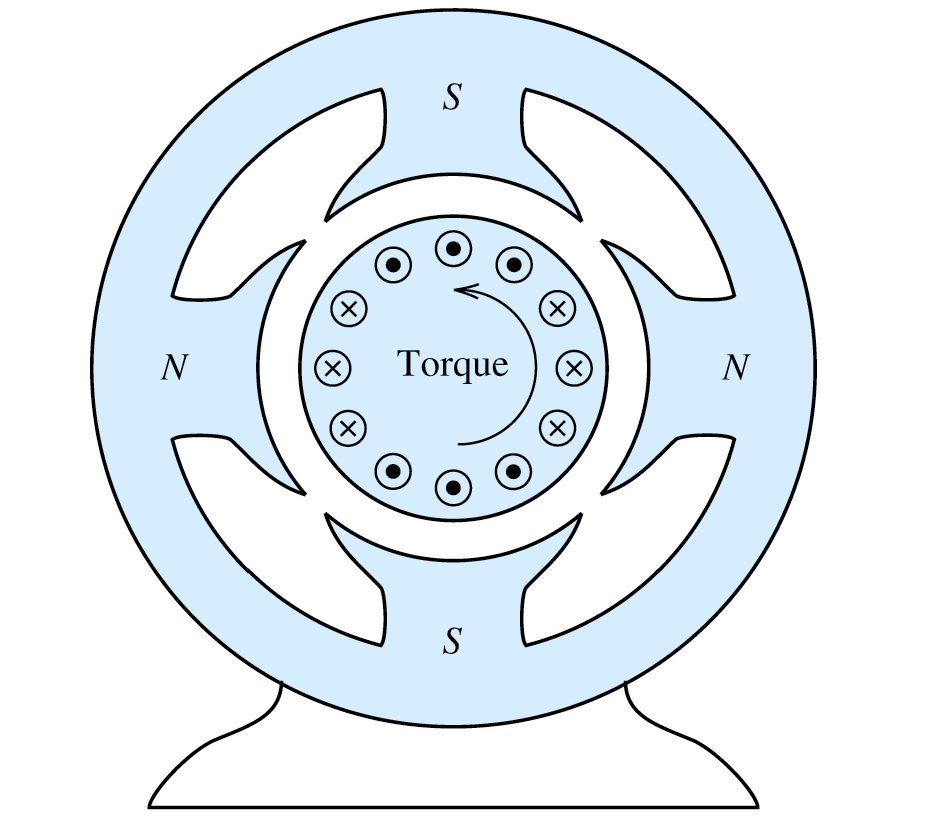
\includegraphics[height=0.5\paperheight]{image49}

                \textbf{4 pole motors}
            \end{center}
        \end{column}
    \end{columns}


\end{frame}

\section{Some simple Newtonian mechanics}

{\fullbackground[scale=0.9,page=2]{ian-simple-newtonian-mechanics.pdf}
    \begin{frame}{Compression \& extension springs}

%Resists with opposing force proportional to extension of movement
%
%
%    \begin{columns}
%        \begin{column}{0.5\linewidth}
%            \begin{center}
%                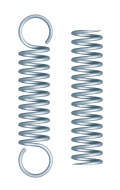
\includegraphics[height=0.3\paperheight]{image52}
%            \end{center}
%        \end{column}
%        \begin{column}{0.5\linewidth}
%            TBD
%        \end{column}
%    \end{columns}
%
%where
%
%f is force in N
%
%k is the spring constant in N/m

\end{frame}
}


{\fullbackground[scale=0.9,page=3]{ian-simple-newtonian-mechanics.pdf}
\begin{frame}{Torsional springs}
%
%    \begin{columns}
%        \begin{column}{0.5\linewidth}
%            \begin{center}
%                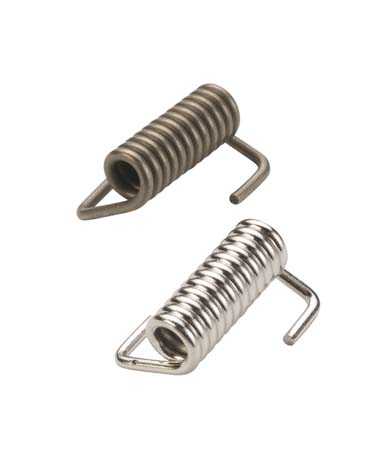
\includegraphics[height=0.3\paperheight]{image54}
%            \end{center}
%        \end{column}
%        \begin{column}{0.5\linewidth}
%            TBD
%        \end{column}
%    \end{columns}
%where
%
%$T$ is torque in $N\cdot m$
%
%$k$ is the spring constant in $\frac{N\cdot m}{rad}$
%
\end{frame}
}

{\fullbackground[scale=0.9,page=4]{ian-simple-newtonian-mechanics.pdf}
\begin{frame}{Dampers and dashpots}

%Resists with opposing force proportional to velocity of movement
%
%
%    \begin{columns}
%        \begin{column}{0.5\linewidth}
%            \begin{center}
%                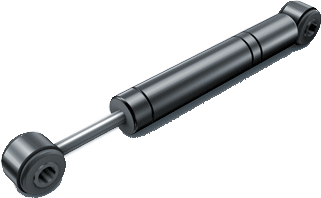
\includegraphics[height=0.3\paperheight]{image57}
%            \end{center}
%        \end{column}
%        \begin{column}{0.5\linewidth}
%            TBD
%        \end{column}
%    \end{columns}
%
%where
%
%$f$ is force in $N$
%
%    $C$ is viscosity in $N\cdot \frac{s}{m}$
%
%Dampers/ shock absorber

\end{frame}
}

{\fullbackground[scale=0.9,page=5]{ian-simple-newtonian-mechanics.pdf}
\begin{frame}{Inertial Mass}
%
%Resists with opposing force proportional to acceleration of movement
%
%    \begin{columns}
%        \begin{column}{0.5\linewidth}
%            \begin{center}
%                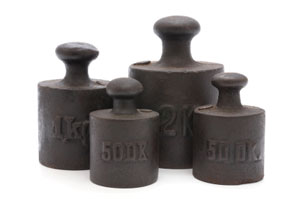
\includegraphics[height=0.3\paperheight]{image60}
%            \end{center}
%        \end{column}
%        \begin{column}{0.5\linewidth}
%            TBD
%        \end{column}
%    \end{columns}
%
%where
%
%$f$ is force in $N$
%
%$m$ is mass in $kg$
%
%$a$ is linear acceleration in $\frac{m}{s^2}$
%
\end{frame}
}

{\fullbackground[scale=0.9,page=6]{ian-simple-newtonian-mechanics.pdf}
\begin{frame}{Moment of Inertia}
%
%Resists with opposing torque proportional to angular acceleration
%
%    \begin{columns}
%        \begin{column}{0.5\linewidth}
%            \begin{center}
%                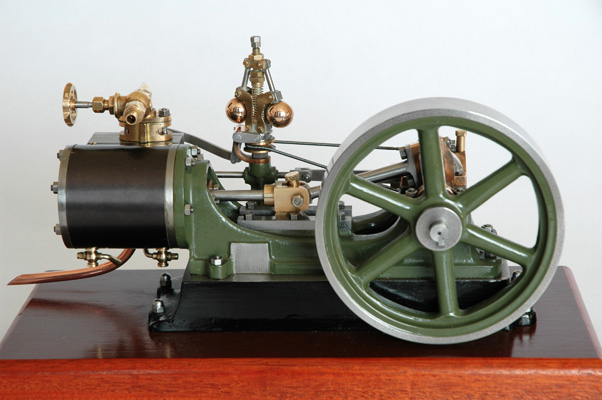
\includegraphics[height=0.3\paperheight]{image62}
%            \end{center}
%        \end{column}
%        \begin{column}{0.5\linewidth}
%            TBD
%        \end{column}
%    \end{columns}
%where
%
%$T$ is torque in $N\cdot m$
%
%$J$ is moment of inertial in $kg \cdot m^2$
%
\end{frame}
}

\section{Differential equation of DC motor rotation}

\begin{frame}{DC motor dynamics}

    \begin{center}
        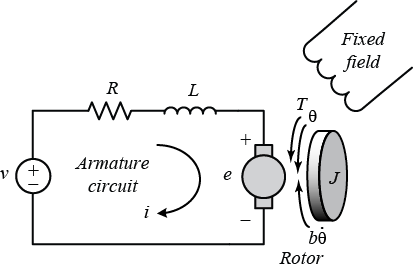
\includegraphics[width=0.5\linewidth]{image63}
    \end{center}

\only<1> {
\begin{itemize}

\item $R$ = Armature resistance (in ohms $\Omega$)
\item $L$ = Armature inductance (in Henrys $H$) % CHECK
\item $J$ = Moment of inertia for the motor rotor ($kg\cdot m^2$)
\item $b$ = Motor viscous friction constant (in $N\cdot m\cdot s$)
\item $K_t$ = Motor torque constant (in $\frac{N\cdot m}{A}$)
\item $K_e$ = Electromotive force constant (in $\frac{V\cdot rad^{-1}}{sec}$) % CHECK
\end{itemize}
}

    \only<2> {
    Motor torque $\tau_m$ is given by $\tau_m = K_t \cdot i(t)$

Mechanical resisting torque $\tau_r$ is given by $\tau_r = b \cdot \dot\theta + J \cdot \ddot\theta$

Under no load, $\tau_m = \tau_r$

Therefore:
\[
    K_t \cdot i(t) = b \cdot \dot\theta + J \cdot \ddot\theta
\]

}
    \only<3> {

\textbf{Kirchhoff's voltage law}: voltage across resistor, inductance and
back EMF balance applied voltage

    \[
        v(t) = i(t) \cdot R + L \cdot \frac{di}{dt} + K_e \cdot \dot\theta
    \]
}
\end{frame}

\begin{frame}{Definition of Laplace transform}

    \only<1>{
The Laplace transform is a linear operator that maps a function $f(t)$ to
$F(s)$.


Specifically:

\[
    F(s) = \mathcal{L}\{f\}(s) =  \mathcal{L}\{f(t)\} = \int^{\inf}_{0} f(t)e^{-st}dt
\]

where $s = \sigma + i\omega$

    Go from a function of a \emph{real} variable (here time $t$) to a complex
    function of a complex variable (frequency, $s$).

}

    \only<2> {

        Why bother?

        Often \textbf{simplifies the process of analyzing the behavior of the
        system}.

        For example, Laplace transformation from the time domain to the
        frequency domain \textbf{transforms differential equations into algebraic
        equations}.
    }
\end{frame}

\begin{frame}{Operations useful for solving differential equations}

\Large

\[
    \mathcal{L} \{f'(t)\} = sF(s) - f(0)
\]


\[
    \mathcal{L} \{f''(t)\} = s^2F(s) - sf(0) - f'(0)
\]


\[
    \mathcal{L} \{\int^{t}_{0}f(t)dt\} = \frac{F(s)}{s}
\]

\vspace{2em}
\small
See
    \href{https://en.wikipedia.org/wiki/Laplace_transform}{Wikipedia}
    for more properties.

\end{frame}

\begin{frame}{Solution using Laplace transformations}

\only<1>{

Taking Laplace transforms of the differential equations that describe
the motor mechanical dynamics:

\[
   K_t \cdot i(t) = b \cdot \dot\theta + J \cdot \ddot\theta
\]

becomes:

\[
    K_t \cdot I(s) = b \cdot s \cdot \theta(s) + J \cdot s^2 \cdot \theta(s)
\]

\[
    I(s) = \frac{s \cdot (b + J \cdot s) \cdot \theta(s)}{K_t}
\]

}

    \only<2> {

Taking Laplace transforms of the differential equations that describe
the motor voltages:

\[
        v(t) = i(t) \cdot R + L \cdot \frac{di}{dt} + K_e \cdot \dot\theta
\]

becomes:

\[
    V(s) = I(s) \cdot (R + L\cdot s) + K_e \cdot s \cdot \theta(s)
\]
}

    \only<3>{

Substituting:

\[
    I(s) = \frac{s \cdot (b + J \cdot s) \cdot \theta(s)}{K_t}
\]


into:

\[
    V(s) = I(s) \cdot (R + L\cdot s) + K_e \cdot s \cdot \theta(s)
\]

Eliminating current $I(s)$ and setting $K_t = K_e = K$ gives:

\[
    \theta(s) = \frac{K}{s \cdot ( (J \cdot s + b) \cdot (L \cdot s+ R) + K^2)} \cdot V(s)
\]

}

\end{frame}

\begin{frame}{Transfer function}

    \begin{columns}
        \begin{column}{0.5\linewidth}

            Result of a transfer response output position for a DC electric motor
            given its input voltage

        \end{column}
        \begin{column}{0.5\linewidth}


            \begin{center}
                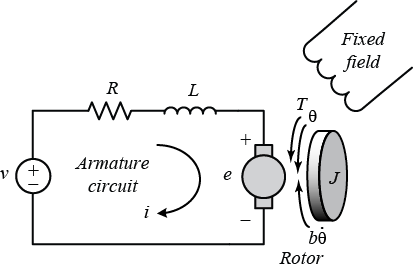
\includegraphics[width=0.9\columnwidth]{image63}
            \end{center}

        \end{column}
    \end{columns}

\[
    \theta(s) = \frac{K}{s \cdot ( (J \cdot s + b) \cdot (L \cdot s+ R) + K^2)} \cdot V(s)
\]

\pause

Can differentiate this expression to get the transfer function for speed

\[
    \dot\theta(s) = \frac{K}{(J \cdot s + b) \cdot (L \cdot s + R) + K^2} \cdot V(s)
\]


\end{frame}

%%%%%%%%%%%%%%%%%%%%%%%%%%%%%%%%%%%%%%%%%%%%%%%%%%%%%%%%%%%%%%%%%%
\section{Brushless DC motors}

{\fullbackground[scale=0.9,page=2]{ian-brushless-dc-motors.pdf}
\begin{frame}{Problems of mechanical commutation}

%Can get potential difference across commutator segments
%
%\begin{itemize}
%
%\item Can get potential difference across commutator segments
%\item Commutation shorts out the commutator segments
%\item Arcing and sparkling at the brushes
%\item Brushless electronic switching solves this issue
%\end{itemize}

\end{frame}
}

{\fullbackground[scale=0.9,page=3]{ian-brushless-dc-motors.pdf}
\begin{frame}{Brushless DC Motor}

%This motor type looks like DC brushed motor turned inside out!
%
%\begin{itemize}
%
%\item This motor type looks like DC brushed motor turned inside out!
%\item In an EC (brushless) motor, commutation is performed electronically to
%  eliminate brushes
%\item The stator generally consists of several coils
%\item Current flow in the stator coils creates magnetic field
%\item This forces the permanent magnet rotor turn
%\item The rotor can be forced to rotate continuously by switching on current
%  in the stator coils in the appreciate sequence thereby generating a
%  sequenced magnetic field
%\item All brushless motors require a controller to work that must perform
%  the commutation operation
%\end{itemize}

\end{frame}
}

{\fullbackground[scale=0.9]{image81}
\begin{frame}{Typical brushless motor}

\end{frame}
}


{\fullbackground[scale=0.9,page=5]{ian-brushless-dc-motors.pdf}
\begin{frame}{How do brushless motors work?}

%\begin{itemize}
%\item Electronic commutation is used to switch current in the stator could
%  so that the rotor is forced to rotate
%\item There is often a control magnet is in line with the poles of the large
%  magnet in the motor to identify rotor angle so that the controller can
%  switch current into the appropriate coils
%\item As it turns Hall sensors are stimulated by the magnetic flux.
%\item The Hall sensors are used to tell the controller what the orientation
%  is of the magnet with respect to the three winding phases.
%\item Current in the stator coils is turned on and off in sequence creating
%  motion from pole to pole.
%\end{itemize}

\end{frame}
}

{\fullbackground[scale=0.9,page=6]{ian-brushless-dc-motors.pdf}
\begin{frame}{Block commutation}

%\begin{itemize}
%\item
%\end{itemize}
%
%\_
%
%HS3
%
%HS1
%
%HS2
%
%controller
%
%power stage
%
%(MOSFET)
%
%phase 1
%
%phase 2
%
%phase 3
%
%EC motor
%
%(magnet, winding, sensor)
%
%rotor position feedback
%
%commutation
%
%logics
%
    \note{

\textbf{On the right} we have a schematic \textbf{cross section of a
maxon EC motor} with 2 pole permanent magnet in the center, the three
phase winding and the three Hall sensors placed at 120°. For simplicity
we assume the Hall sensors to probe the power magnet directly.

\textbf{On the left} we have the \textbf{commutation electronics} which
is fed with a DC supply voltage. There is a power bridge made of 6
MOSFETs. Three of them are needed to contact the motor phases to the
positive supply voltage. The lower three MOSFETs make the contact to the
supply ground. The power bridge is controlled by a commutation logic
that evaluates the Hall sensor signals and, accordingly, switches the
power on the three motor phases.

\textbf{Comments on the animation:}

In this starting position the Hall sensors give the following signal:
HS1 has just switched to a high state, HS2 is low and HS3 is high.

The commutation logic knows that for this signal combination and
clockwise motor rotation the current must flow from phase 1 to 2 and
powers the respective two MOSFETs.

The winding produces a magnetic field and the magnetic rotor tries to
align.

After 60° the HS3 starts seeing the south pole. Its output switches to
low and the commutation logic switches the current from phase 1 to 3.
The field of the winding advances by 60° and the rotor continues to
rotate.

Again after 60° the Hall sensor pattern changes, HS2 switches to a high
output level. Accordingly the electronics commutates the current to flow
from phase 2 to 3. Again the field of the winding advances by another
60° and the rotor continues.

And so on \ldots{} . After 6 commutation intervals we are back at the
initial configuration and the rotor has accomplished one turn.

}

\end{frame}

}

{\fullbackground[scale=0.9,page=7]{ian-brushless-dc-motors.pdf}
\begin{frame}{Brushless motor for RC aircraft}

\end{frame}
}

{\fullbackground[scale=0.9,page=8]{ian-brushless-dc-motors.pdf}
\begin{frame}{Maxon EC brushless motor}

%Permanent magnet
%
%Special Winding
%
%Rotating part -- permanent magnet
%
%Hall sensors
%
%Control Magnet
%
%Case / Magnetic
%
%return

\end{frame}

}

{\fullbackground[scale=0.9,page=9]{ian-brushless-dc-motors.pdf}
\begin{frame}{Maxon EC flat brushless motor}

%Multi pole motor
%
%Flat design gives more torque as the flux is acting further from the
%centre of rotation

\end{frame}

}

{\fullbackground[scale=0.9,page=10]{ian-brushless-dc-motors.pdf}
\begin{frame}{Advantages and disadvantages of EC}

%\textbf{Brushed DC motors}
%
%\begin{itemize}
%
%\item Mechanical commutation
%\item Need periodic brush maintenance
%\item Power losses in brushes
%\item Sparking
%\item Can have noisy operation
%\item Linear torque characteristic at lower
%\item Change direction by changing voltage polarity
%\item Controller not always needed
%\end{itemize}
%
%\textbf{EC motors}
%
%\begin{itemize}
%
%\item Electronic commutation
%\item Low or no maintenance
%\item Less power loss
%\item No sparking
%\item Quieter operation
%\item More linear torque characteristic
%\item Change direction by changing switching sequence
%\item Always needs drive controller circuitry
%\item Requires sensors
%\item Higher reliability \& efficiency
%\item Stator on outside -- better for heat dissipation
%\item Longer life
%\item More expensive
%\end{itemize}

\end{frame}
}

%\section{Some other motors}
%
%\begin{frame}{Wound field motors}
%
%\begin{itemize}
%
%\item What happens if we apply AC to a permanent magnet DC motor?
%\end{itemize}
%
%\end{frame}
%
%\begin{frame}{Motor with stator winding}
%
%\end{frame}
%
%\begin{frame}{Shunt motor}
%
%\begin{itemize}
%\item Like DC motor but with electromagnet to generate static field
%\item Armature and field windings are connected in parallel
%\item Separate current through stator and armature
%\item Low Starting Torque
%\item Good Speed Regulation
%\item Used for fixed speed applications, windscreen wipers, fans
%\end{itemize}
%
%\end{frame}
%
%\begin{frame}{Shunt motor}
%
%Consider motor behavior under load:
%
%\begin{itemize}
%
%\item On application of load speed will reduce
%\item But this reduced armature EMF
%\item Therefore armature current rises
%\item Therefore torque increases
%\item So speed increases too
%\item Therefore system can do some self regulation of speed
%\item Much like permanent magnet DC motor!
%\end{itemize}
%
%\end{frame}
%
%\begin{frame}{Series motor}
%
%\begin{itemize}
%
%\item Armature and field windings are connected in series
%\item Same current goes through both
%\item High Starting Torque
%\item As the speed builds up so does the back EMF, reducing the current,
%  which causes a reduction in torque
%\item Poor Speed Regulation
%\item Used for starting heavy, industrial, high torque loads such as cranes,
%  hoists, elevators, trolleys and conveyors
%\item Cannot operate safely in an unloaded condition
%\end{itemize}
%
%\end{frame}
%
%\begin{frame}{Universal Motors}
%
%\begin{itemize}
%
%\item Series motor
%\item Uses field coils and not permanent magnets
%\item AC and DC operation
%\item As current direction changes it changes field direction on stator
%  field and also armature
%\item So always rotates in same direction independent of applied current
%  direction
%\end{itemize}
%
%\end{frame}

\begin{frame}{Images and drawings from:}

\begin{itemize}

\item Images and drawings from:
\item Maxon Motor
\item http://ctms.engin.umich.edu/
\item \url{http://hyperphysics.phy-astr.gsu.edu/}
\item Wikipedia
\item Internet in general
\end{itemize}

\textbf{Please respect copyright}

\end{frame}


\begin{frame}{}
    \begin{center}
        \Large
        That's all, folks!\\[2em]
        \normalsize
        Questions:\\
        Portland Square A216 or \url{severin.lemaignan@plymouth.ac.uk} \\[1em]

        Slides:\\ \href{https://github.com/severin-lemaignan/module-mobile-and-humanoid-robots}{\small github.com/severin-lemaignan/module-mobile-and-humanoid-robots}

    \end{center}
\end{frame}



\end{document}
